\chapter[Solução Geral]{Solução Geral}
\section{Escopo}
% Descrever projeto e especificar protótipos caso exista
O projeto PillWatcher consiste na construção de um dispensador automático de medicamentos sólidos, o qual terá a função de armazenar e realizar a separação da dose medicamentosa individual nos horários pré-estabelecidos pelo médico. Além do mais, o projeto possuirá uma aplicação \textit{mobile} e um conjunto de microsserviços únicos com o servidor de gerenciamento da interface com o usuário e o gerenciamento da coleta de dados.

Existirá a comunicação entre o dispositivo e o aplicativo, uma vez que, este será elaborado para realizar o cadastro de enfermeiros, pacientes e medicamentos, além de enviar avisos quando se aproxima do horário da medicação. O aplicativo informará a quantidade de todos os medicamentos, avisando a reposição quando necessária.

Assim, para realizar a adição dos remédios no dispositivo é necessário retirar os medicamentos sólidos da embalagem, blister ou frasco seguindo um protocolo rígido de higiene com a utilização de equipamentos de proteção individual (EPIs) e despejá-los separadamente por lote e validade em cada contêiner.

O compartimento superior do dispositivo contará com uma entrada para realizar o abastecimento de medicamentos no estoque de contêineres. Enquanto que, no compartimento frontal, existirá uma saída para a retirada dos recipientes com a medicação correta para cada paciente. Entretanto, é necessária uma autenticação do corpo técnico de médicos, enfermeiros e cuidadores das clínicas geriátricas para permitir o acesso a esses compartimentos.

Visando uma melhor compreensão do projeto, foram elaboradas soluções particulares de cada área do projeto afim de garantir a elaboração correta do produto final.

\section{Lista É/ Não É}
A Lista É/ Não É que define o projeto PillWatcher encontra-se no Apêndice \ref{Lista_app}

%% Rich Picture
\section{Rich Picture}
\label{richpiture_software}

Os \textit{Rich Pictures} são modelos que permitem a análise de problemas e a expressão de ideias. O \textit{Rich Picture} auxilia na compreensão da complexidade do ambiente no qual a aplicação de desenvolvimento está operando, e consequentemente fornece uma visão geral do problema a ser resolvido.


Na Figura \ref{fig:Communication_between_components} é apresentado o fluxo de interação entre os componentes de software e os componentes eletrônicos que serão inseridos no desenvolvimento do dispensador, bem como a especificação da interação entre os módulos de \textit{Front-end} e \textit{Back-end} na aplicação e sua comunicação com o banco de dados.

\subsection{Comunicação Entre Componentes}
\begin{figure}[H]
    \centering
    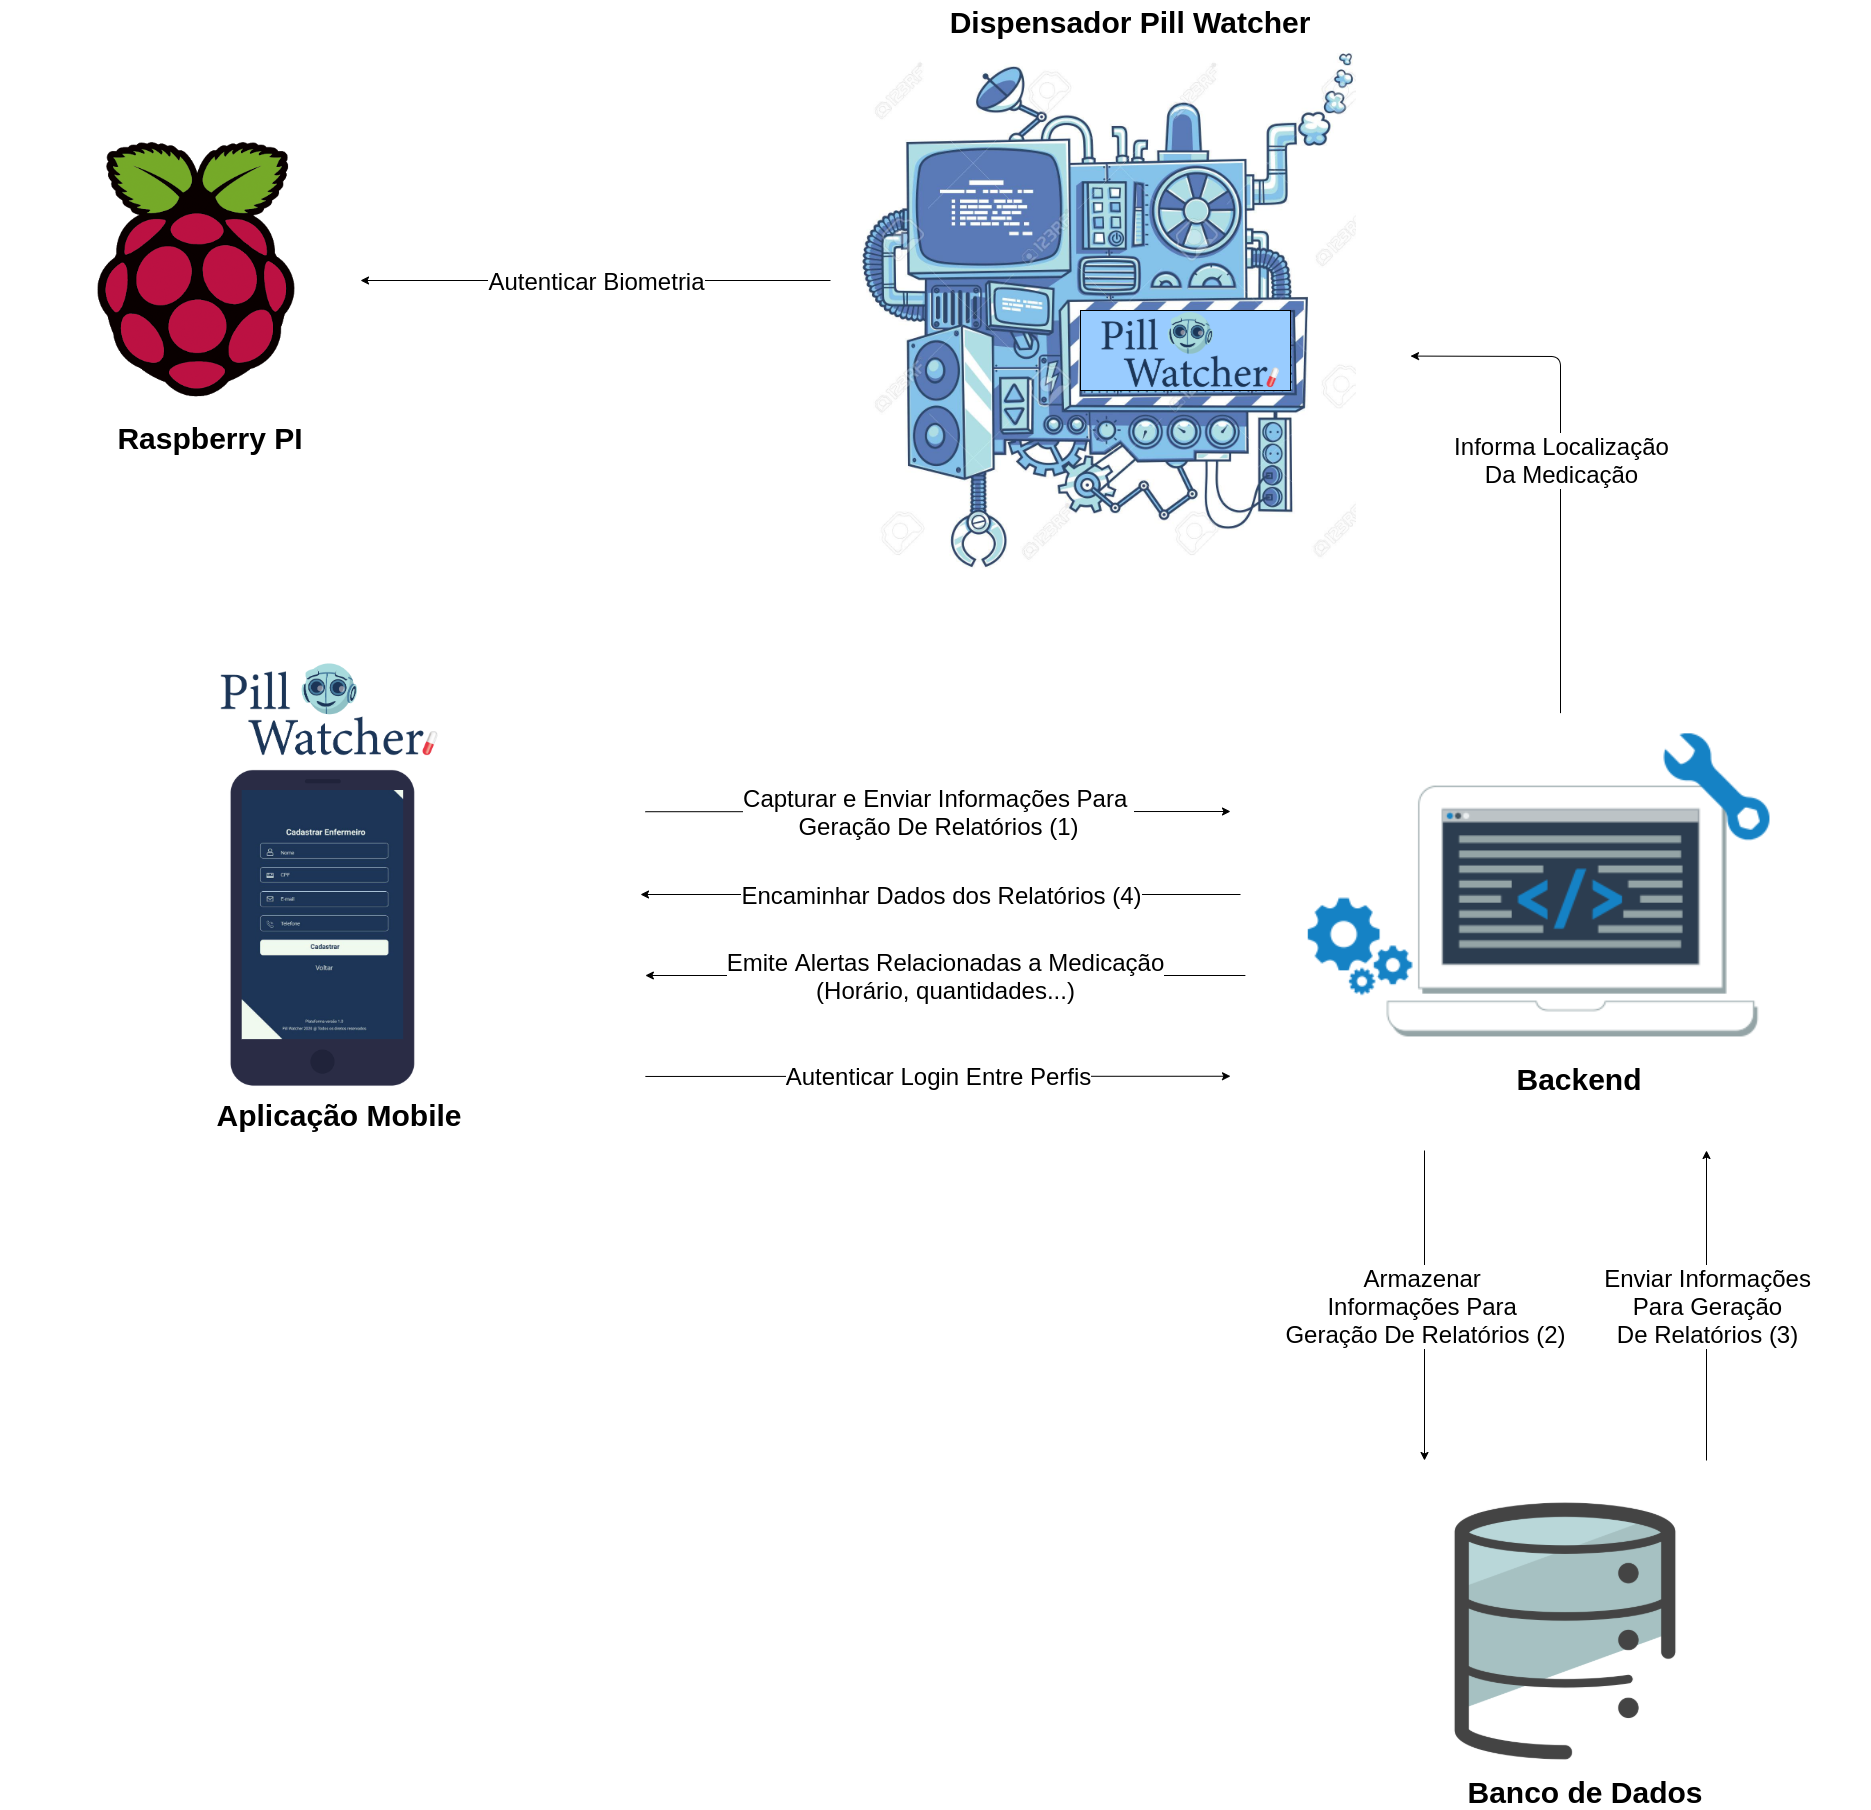
\includegraphics[width=0.85\textwidth]{figuras/Comunicação Entre Componentes.png}
    \caption{Comunicação entre componentes de software e eletrônicos}
    \label{fig:Communication_between_components}
\end{figure}

No esquema seguinte, apresentado na Figura \ref{fig:Communication_between_entities}, é demonstrado os relacionamentos entre os usuários envolvidos e a aplicação, bem como suas principais funcionalidades implementadas.

\subsection{Comunicação Entre Entidades e Solução de Software}
\begin{figure}[H]
    \centering
    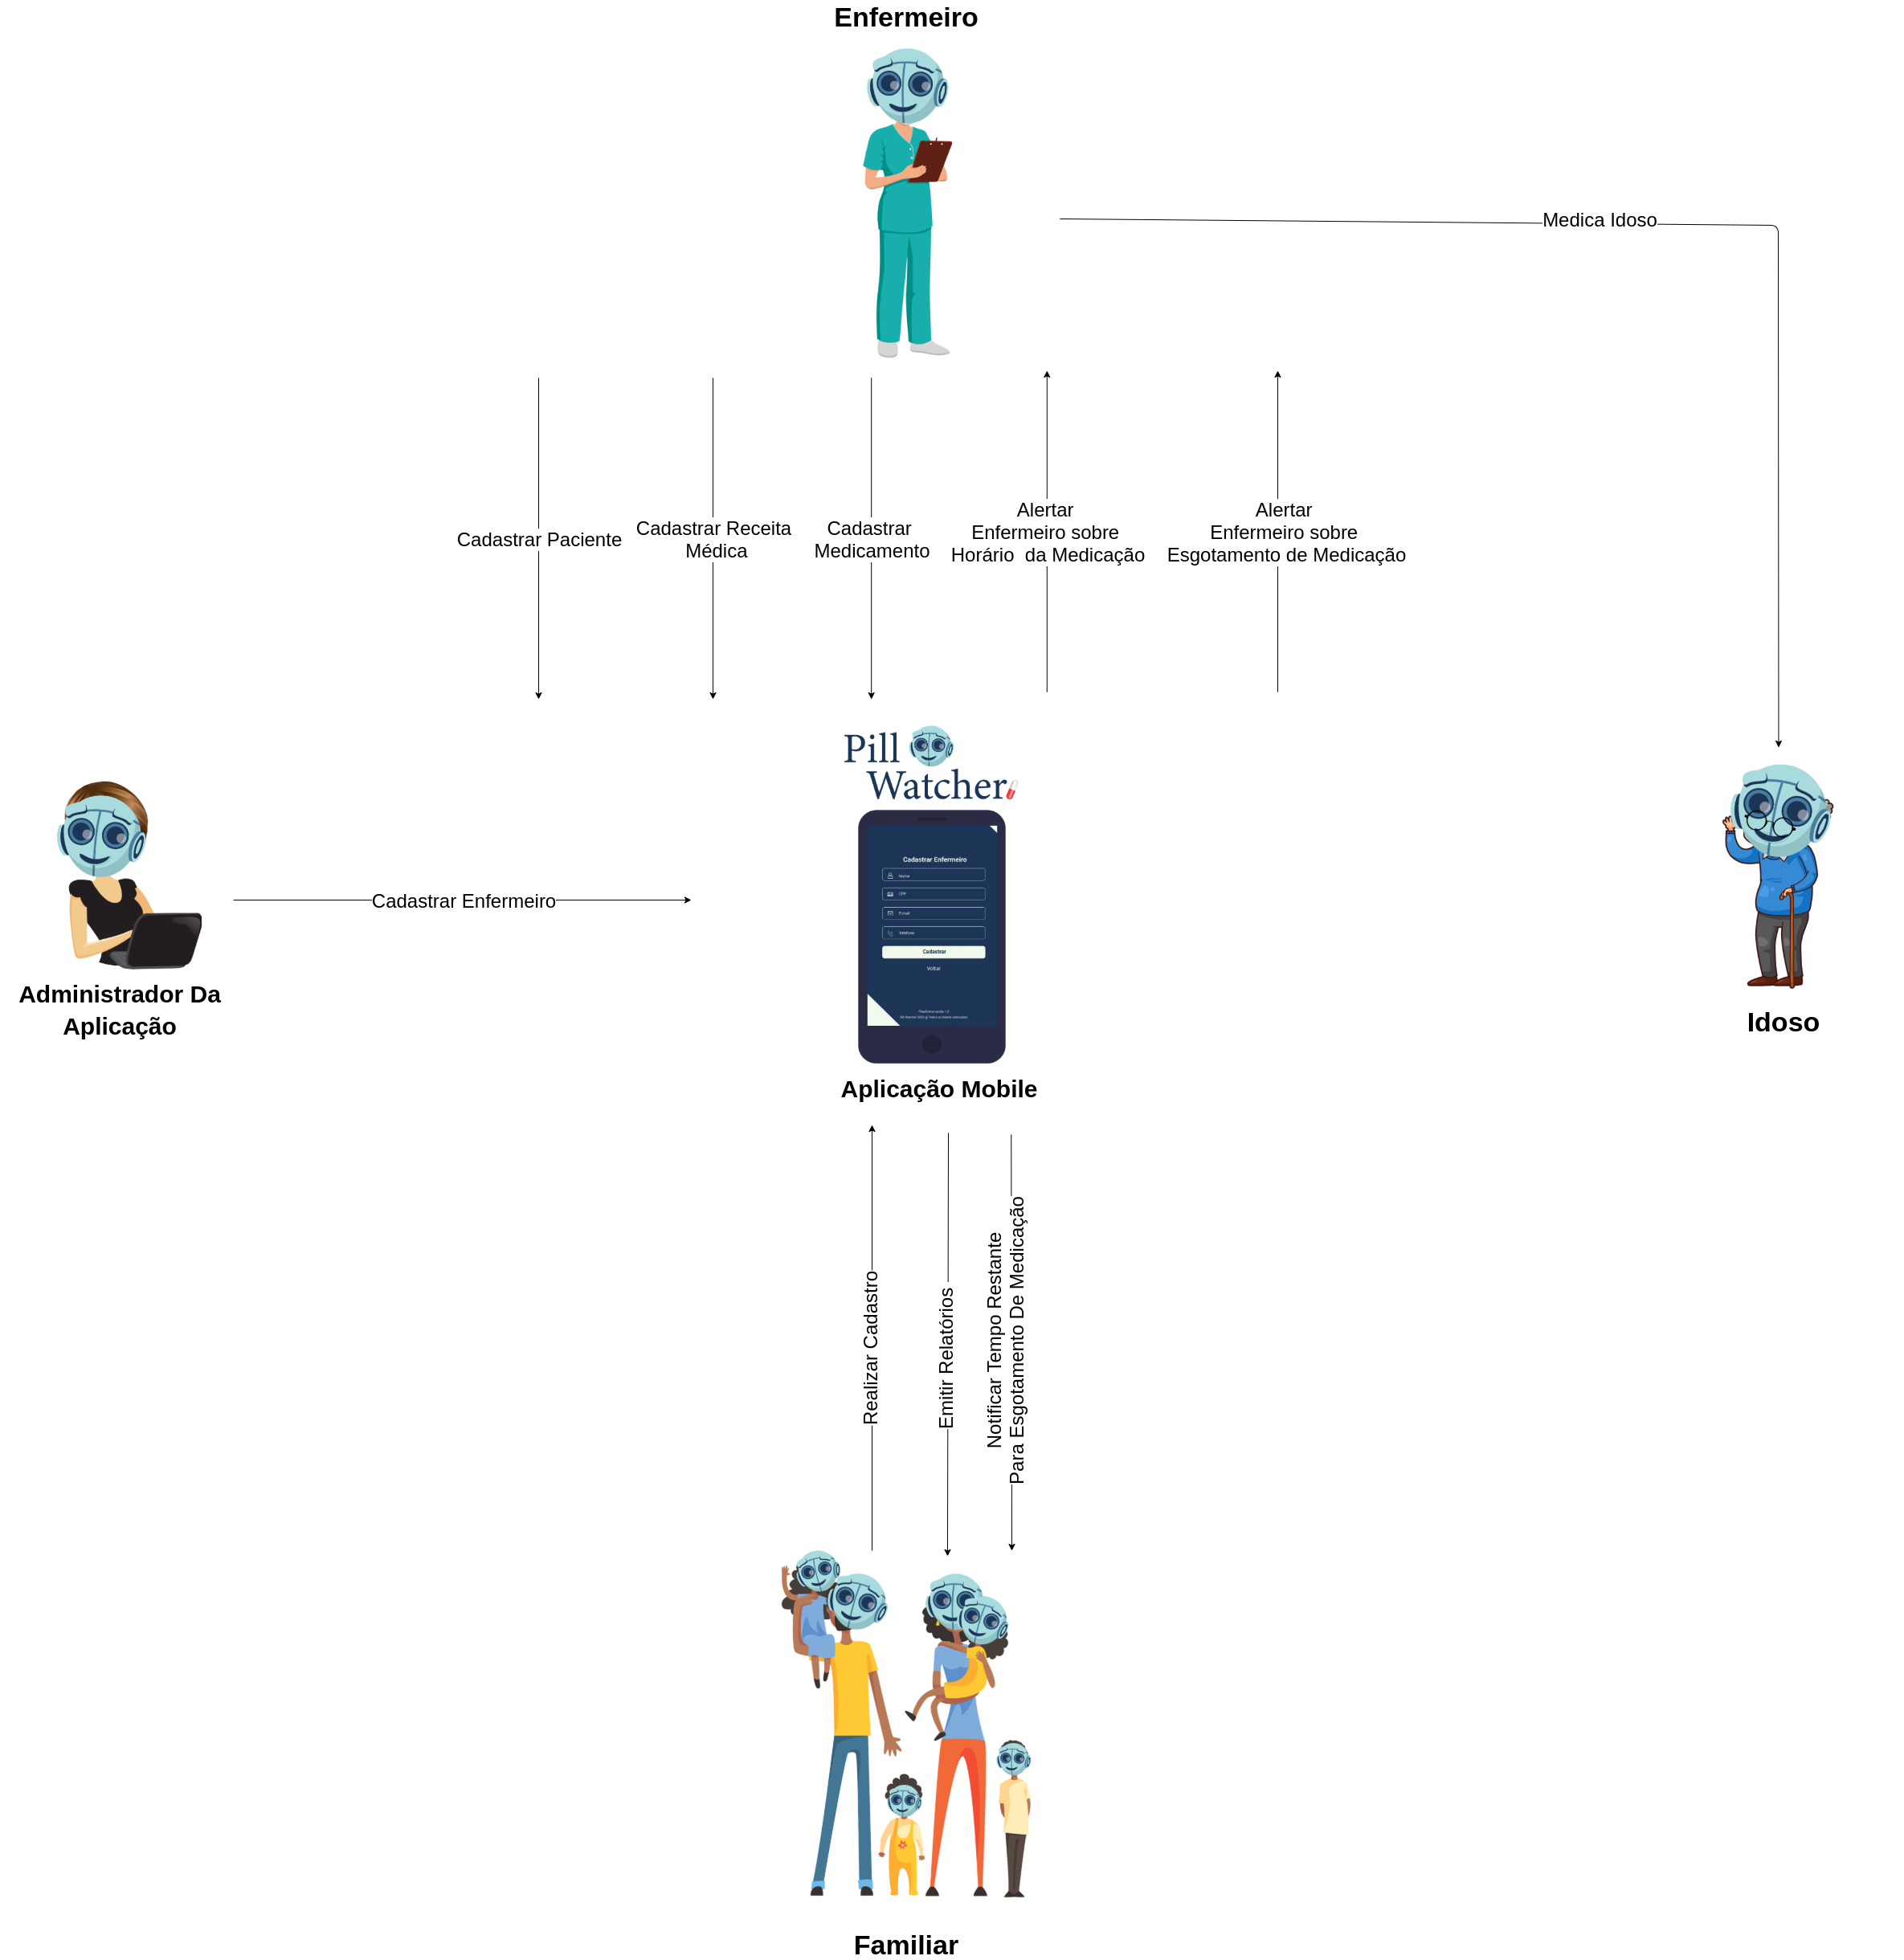
\includegraphics[width=\textwidth]{figuras/Comunicação Entre Entidades e Solução De Software.png}
    \caption{Comunicação Entre Entidades e Solução de Software}
    \label{fig:Communication_between_entities}
\end{figure}